\documentclass[11pt,a4paper]{article}
\usepackage[margin=23mm]{geometry}
\usepackage[T1]{fontenc}
\usepackage{lmodern}
\usepackage{booktabs,graphicx,listings,xcolor,float,caption,amsmath,needspace}
\usepackage[hidelinks]{hyperref}
\usepackage{xurl}
\hypersetup{pdftitle={SD6103 Merged Tasks 3 and 4: 2023-2025},pdfauthor={SD6103 Project Group}}
\definecolor{codebg}{rgb}{0.97,0.97,0.97}
\definecolor{codeframe}{rgb}{0.75,0.75,0.75}
\lstset{language=SQL,basicstyle=\ttfamily\fontsize{9}{10.96}\selectfont,
 keywordstyle=\color{blue!70!black},stringstyle=\color{red!55!black},
 commentstyle=\color{gray},backgroundcolor=\color{codebg},rulecolor=\color{codeframe},
 frame=single,framerule=0.35pt,framesep=3pt,breaklines=true,breakatwhitespace=false,
 columns=fullflexible,keepspaces=true,showstringspaces=false,upquote=true,tabsize=4,
 aboveskip=7pt,belowskip=9pt,morekeywords={FILTER,WITHIN,EXTRACT,TRUE,FALSE,IS,NULLIF}}
\captionsetup{font=small,skip=7pt}
\setlength{\parindent}{0pt}
\setlength{\parskip}{5pt}
\setlength{\textfloatsep}{12pt}
\setlength{\intextsep}{12pt}
\clubpenalty=10000
\widowpenalty=10000
\raggedbottom
\setcounter{section}{3}
\begin{document}
\section{Task 3: Queries and Results}
\begin{samepage}All six queries use one common housing-transaction scope: \textbf{1 January 2023 to 31 December 2025}, three complete calendar years and 36 months. The six logical base relations preserve the final ER entities and add one distance-band lookup: \texttt{town}, \texttt{hdb\_flat}, \texttt{resale\_transaction}, \texttt{hawker\_centre}, \texttt{nearby}, and \texttt{proximity\_level}. An HDB-flat record represents a geocoded block address, rather than an individually identified housing unit. The executable SQL includes explanatory trailing comments.\par\end{samepage}

\Needspace{10\baselineskip}\subsection{Derived proximity view and data scope}
\begin{samepage}All queries use a lower bound of \texttt{2023-01-01} (inclusive) and an upper bound of \texttt{2026-01-01} (exclusive). The next-year boundary includes every month through December 2025. The same bounds appear in every query and in a table check constraint. Both stages of Q3 use the same period. All 36 calendar months are present; no matched transaction in this instance falls outside that interval.\par\end{samepage}

\begin{samepage}The \texttt{nearby\_classified} view derives near [0,500), medium [500,1000), and far [1000,2000] metres from stored great-circle distance. The final upper bound is inclusive. A numeric proximity rank preserves logical order. The view reads the three-row proximity lookup; the lookup is a logical implementation detail rather than a new conceptual ER entity. Its non-overlap constraint prevents one stored link matching two bands. Coordinates and hawker attributes remain the supplied reference snapshots, not historical reconstructions for each sale date.\par\end{samepage}

\lstinputlisting{../sql/02_view.sql}
\begin{table}[H]\centering\small
\begin{tabular}{lrl}
\toprule
Measure & Value & Definition \\
\midrule
Raw sales in the selected period & 78,670 & January 2023 - December 2025 \\
Matched transactions & 78,670 & No in-period geocode exclusions \\
hdb\_flat records & 9,385 & Participating block-address records \\
Hawker centres & 129 & 81 yes, 23 no, 25 unknown \\
nearby links & 40,354 & Retained pairs at or below 2,000 m \\
Observed sale months & 36 & January 2023 - December 2025 \\
\bottomrule
\end{tabular}
\caption{Database instance used for all six queries; only 2023-2025 transactions are included.}
\end{table}
\begin{samepage}All numerical results were executed in PostgreSQL 18.6 through PGlite 0.5.10 (WebAssembly), then independently recomputed with pandas. Figures 1--6 show actual result exports in an generated result-table viewer; they are not pgAdmin captures. Prices are nominal SGD. Native PostgreSQL timings and genuine pgAdmin captures are not established by this run. The project guide requires approval for alternative tools; such approval has not been established here.\par\end{samepage}

\Needspace{10\baselineskip}\subsection{Q1: Price per square metre across towns}
\begin{samepage}The query selects 4 ROOM and 5 ROOM transactions from January 2023 through December 2025, then averages each sale's resale price divided by floor area. Each transaction has equal weight; the measure is not total price divided by total area. The result contains 52 town/type groups and 52,280 qualifying sales.\par\end{samepage}

\Needspace{7\baselineskip}\lstinputlisting{../sql/queries/Q1.sql}
\begin{table}[H]\centering\small
\begin{tabular}{llrr}
\toprule
Town & Type & Mean SGD/m2 & Sales \\
\midrule
Central Area & 5 ROOM & 11,680.14 & 60 \\
Central Area & 4 ROOM & 10,714.41 & 211 \\
Queenstown & 4 ROOM & 9,944.81 & 784 \\
Queenstown & 5 ROOM & 9,254.12 & 186 \\
\bottomrule
\end{tabular}
\caption{Q1: four highest of 52 groups, January 2023 - December 2025.}
\end{table}
\begin{figure}[H]\centering
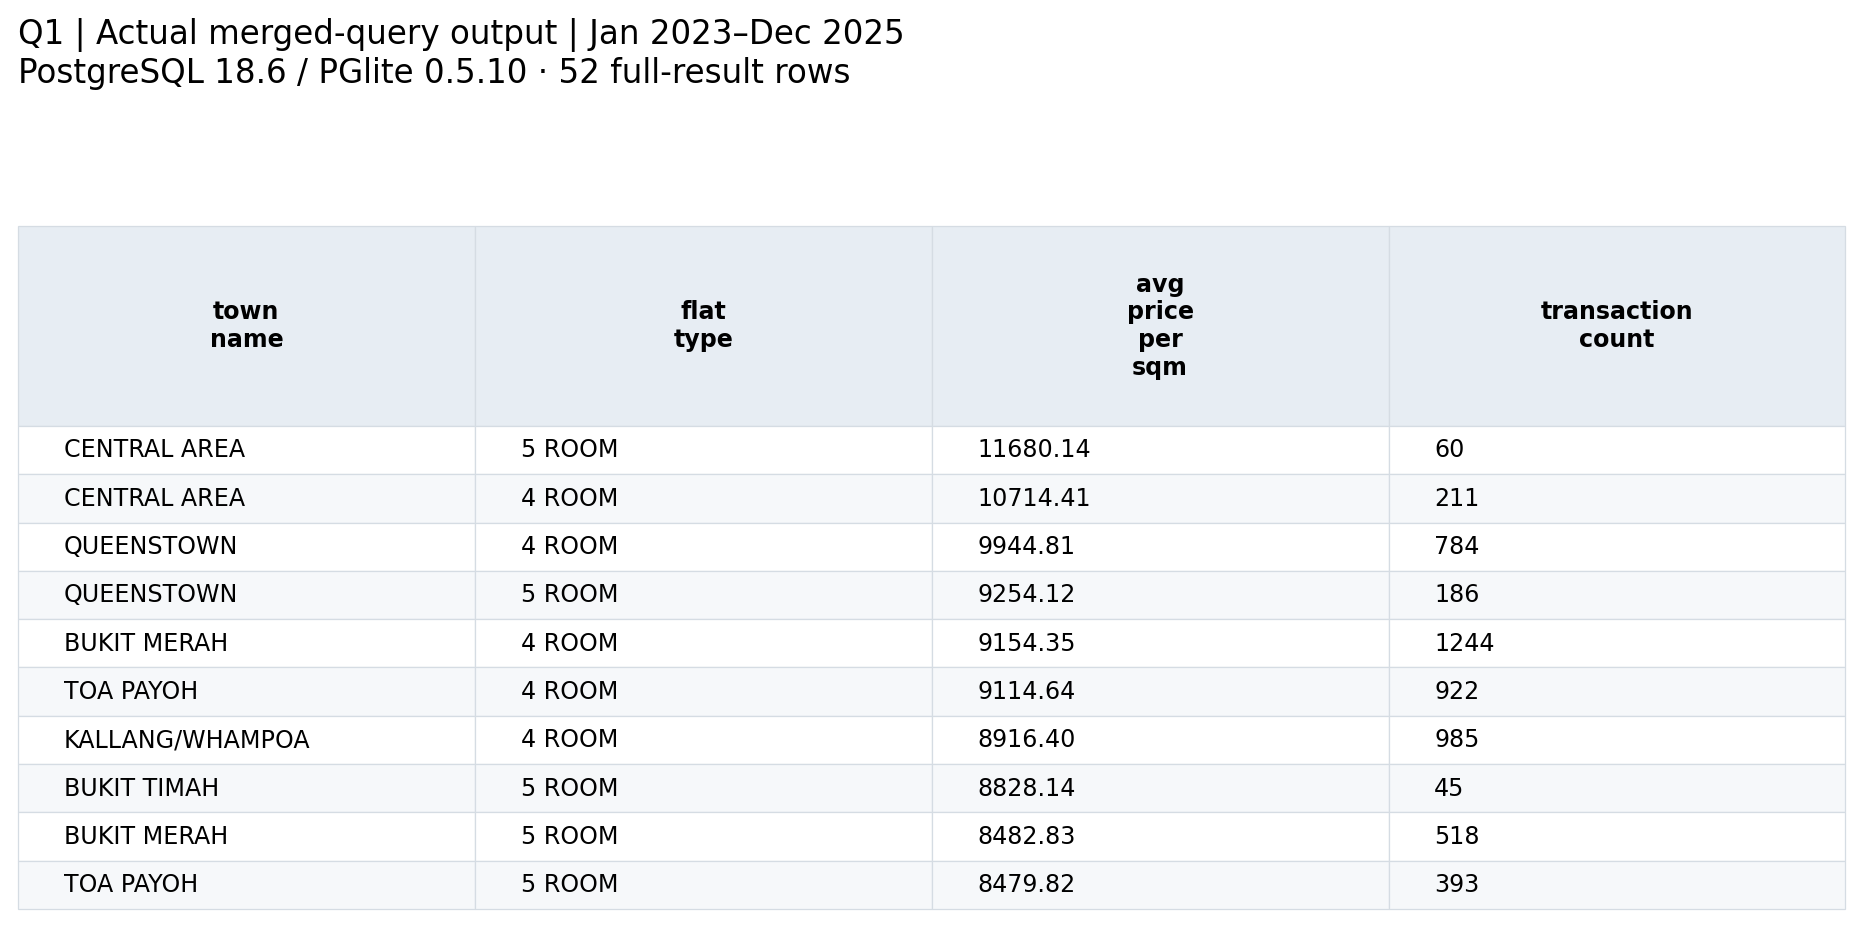
\includegraphics[width=0.94\linewidth,height=8.6cm,keepaspectratio]{../evidence/figures/Q1_result.png}
\caption{Q1 result excerpt: first ten of 52 groups in SQL output order; scope 2023-2025.}\end{figure}
\begin{samepage}\textbf{Insight.} Central Area 5 ROOM has the highest mean at SGD 11,680.14/m2 (60 sales), followed by Central Area 4 ROOM at SGD 10,714.41/m2. This describes the selected three-year period. Lease, floor, flat model and building composition remain uncontrolled, so the ranking is not a causal measure of town value.\par\end{samepage}

\Needspace{10\baselineskip}\subsection{Q2: Remaining lease and transaction price}
\begin{samepage}Each in-period sale enters one disjoint bucket: below 600 months, 600 to below 840 months, or at least 840 months. For each town/bucket, the query returns the continuous median price, mean price per square metre and volume. The 62 output groups partition all 78,670 transactions. Bucket order is numerical, rather than alphabetical.\par\end{samepage}

\Needspace{7\baselineskip}\lstinputlisting{../sql/queries/Q2.sql}
\begin{table}[H]\centering\small
\begin{tabular}{llrrr}
\toprule
Town & Lease bucket & Median SGD & Mean SGD/m2 & Sales \\
\midrule
Ang Mo Kio & < 50 years & 436,944.00 & 5,995.75 & 14 \\
Ang Mo Kio & 50 to < 70 years & 438,888.00 & 5,869.39 & 2,428 \\
Ang Mo Kio & 70+ years & 900,000.00 & 9,280.82 & 634 \\
\bottomrule
\end{tabular}
\caption{Q2: Ang Mo Kio excerpt from 62 groups, using only 2023-2025 sales.}
\end{table}
\begin{figure}[H]\centering
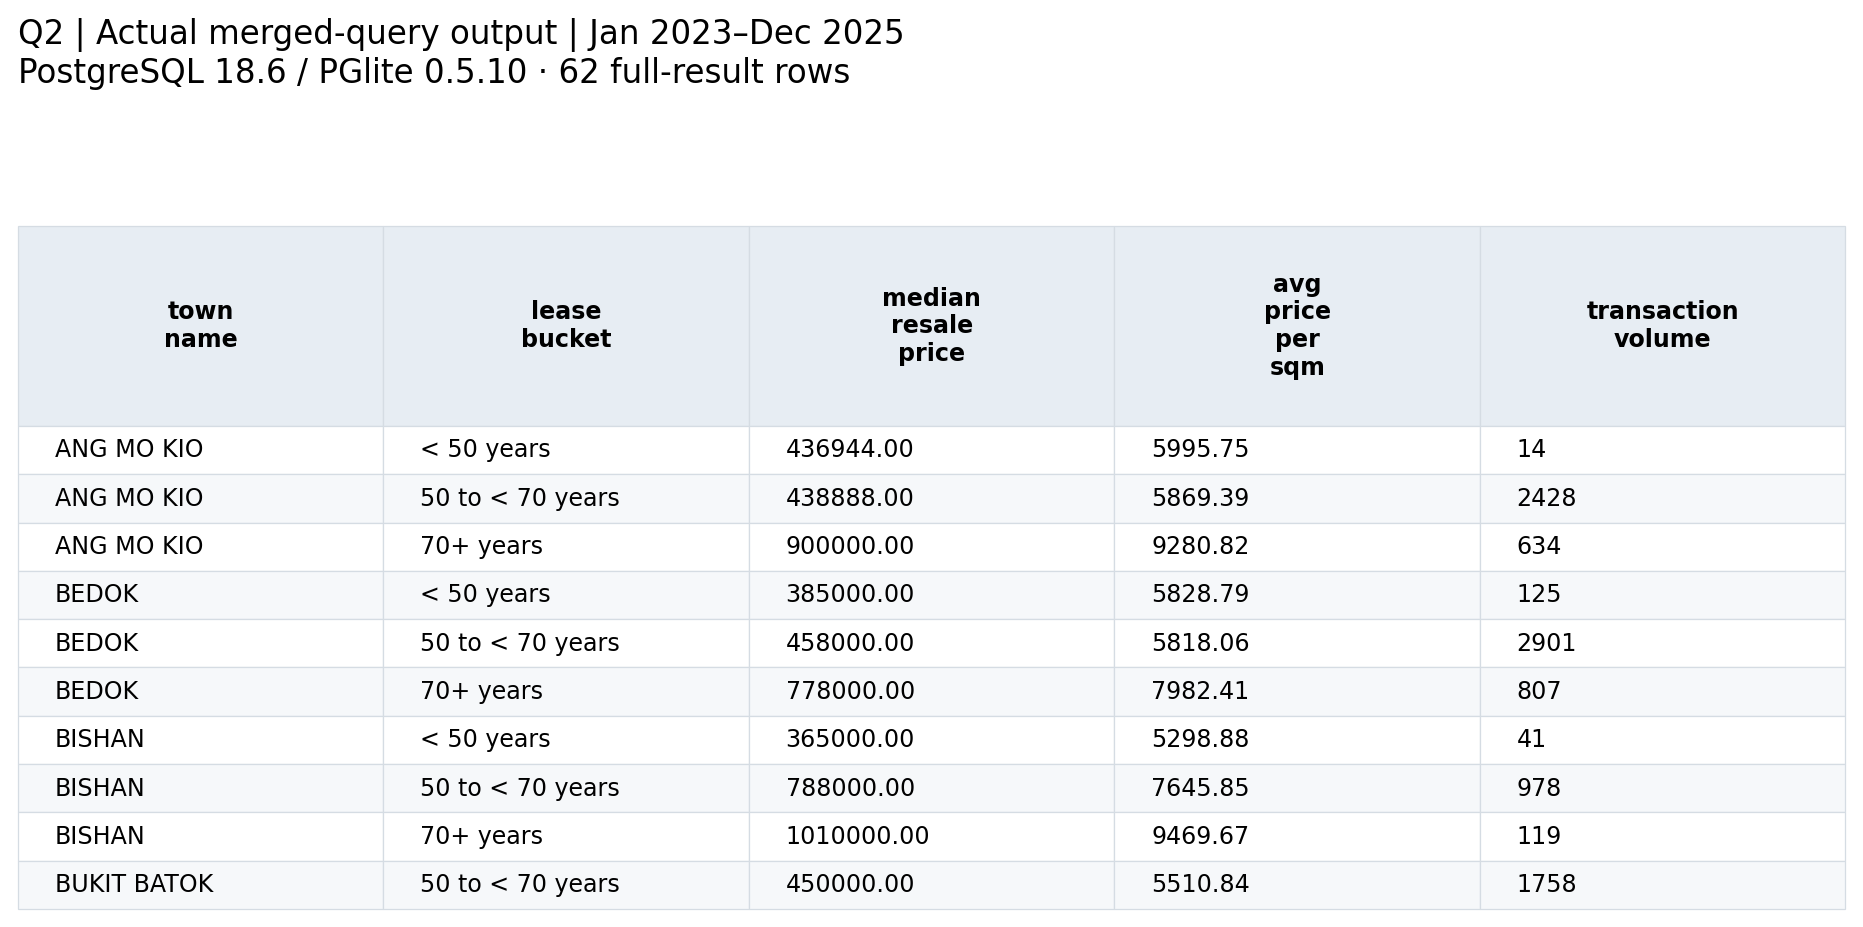
\includegraphics[width=0.94\linewidth,height=8.6cm,keepaspectratio]{../evidence/figures/Q2_result.png}
\caption{Q2 result excerpt: first ten of 62 town/bucket groups, 2023-2025.}\end{figure}
\begin{samepage}\textbf{Insight.} In Ang Mo Kio, the 70+ years group has a median of SGD 900,000 across 634 sales, compared with SGD 438,888 across 2,428 sales in the 50 to below 70 years group. The below-50 group has only 14 sales and a median of SGD 436,944, so its estimate is particularly sensitive to sample composition. Restricting the sale years reduces the earlier historical-price mixing, but differences in flat type, floor area and building cohort remain. The comparison does not isolate a lease effect.\par\end{samepage}

\Needspace{10\baselineskip}\subsection{Q3: Towns with large 3-room flats}
\begin{samepage}The CTE ranks towns by the transaction-weighted mean area of 3 ROOM sales in 2023-2025 and selects ten, with town ID as a tie-break. The outer query keeps the same room type and date bounds, then finds each town's maximum price per calendar year. All three years are complete; the output contains 30 town/year groups.\par\end{samepage}

\Needspace{7\baselineskip}\lstinputlisting{../sql/queries/Q3.sql}
\begin{table}[H]\centering\small
\begin{tabular}{rlrr}
\toprule
Rank & Town & Mean area m2 & 2025 maximum SGD \\
\midrule
1 & Tampines & 71.24 & 698,000.00 \\
2 & Ang Mo Kio & 71.01 & 794,500.00 \\
3 & Bukit Timah & 70.94 & 602,888.00 \\
4 & Jurong East & 70.51 & 558,000.00 \\
5 & Bukit Panjang & 70.37 & 548,888.00 \\
6 & Choa Chu Kang & 69.81 & 530,000.00 \\
7 & Clementi & 69.32 & 740,188.00 \\
8 & Yishun & 68.84 & 620,000.00 \\
9 & Woodlands & 68.71 & 588,000.00 \\
10 & Hougang & 68.32 & 640,000.00 \\
\bottomrule
\end{tabular}
\caption{Q3: ten selected towns and their complete-calendar-2025 maxima.}
\end{table}
\begin{figure}[H]\centering
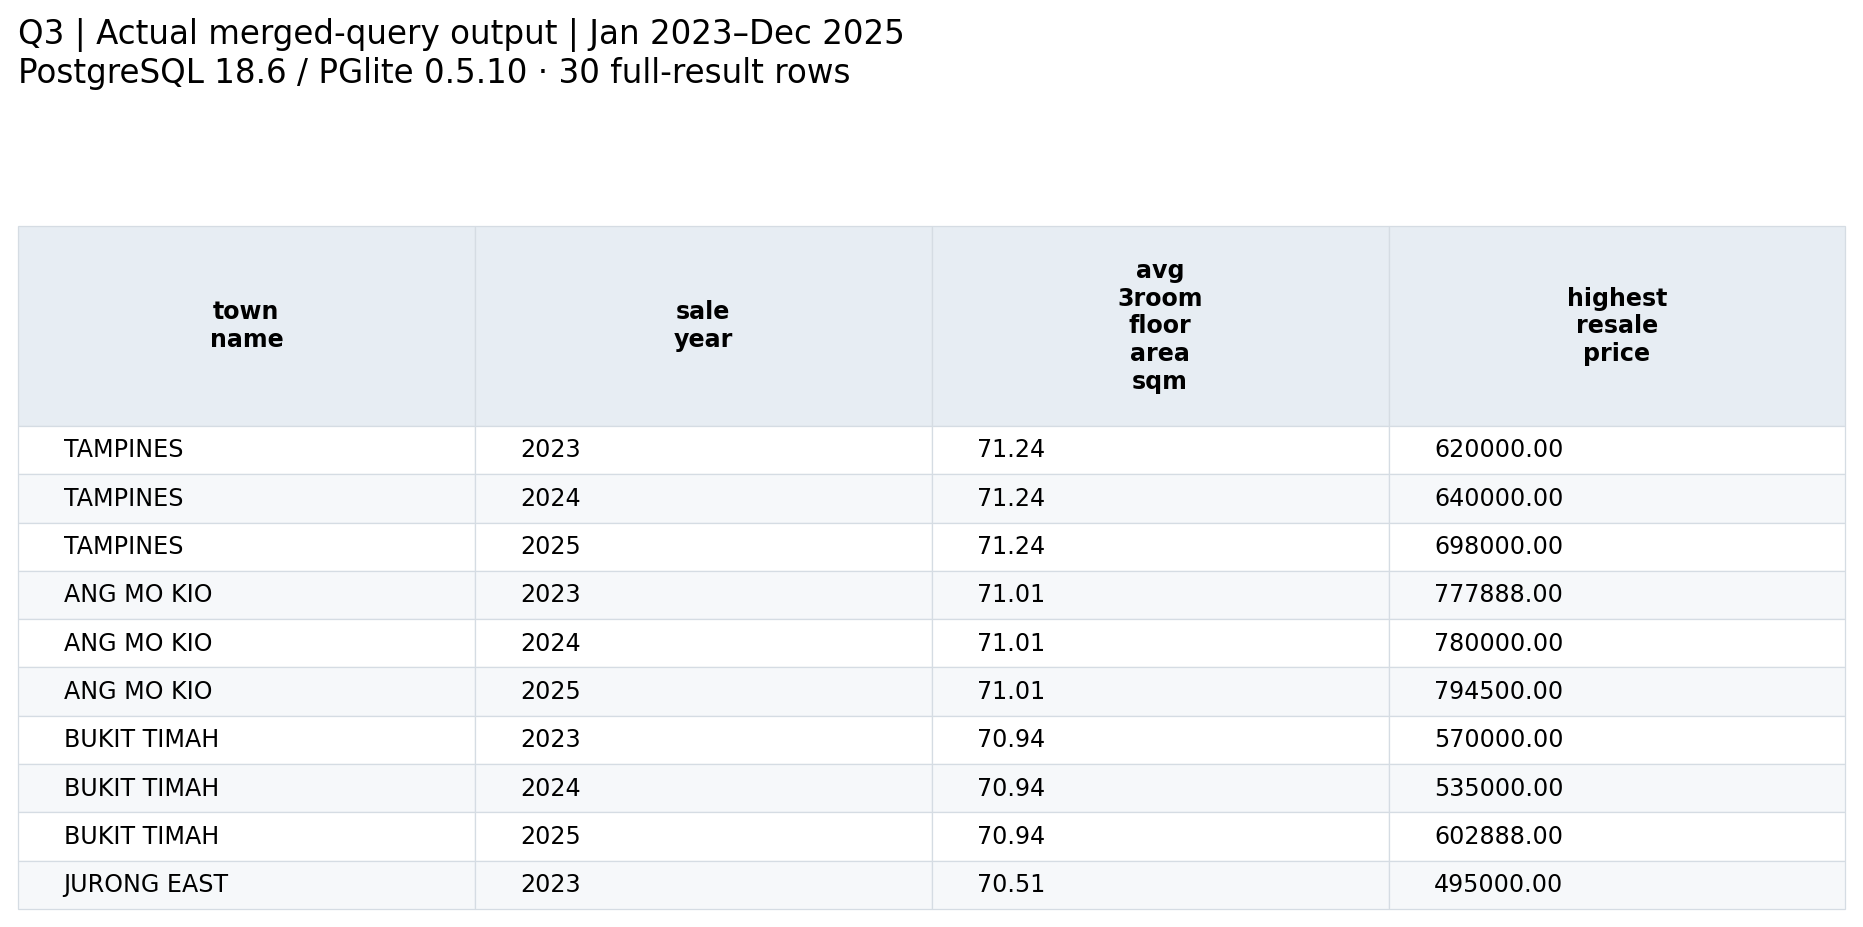
\includegraphics[width=0.94\linewidth,height=8.6cm,keepaspectratio]{../evidence/figures/Q3_result.png}
\caption{Q3 result excerpt from 30 rows: ten towns and three complete calendar years.}\end{figure}
\begin{samepage}\textbf{Insight.} Tampines ranks first with a mean 3 ROOM area of 71.24 m2. The largest annual maximum among selected towns is Clementi in 2024, at SGD 840,000.00. Mean area and maximum price describe different features of the population. A yearly maximum is an exceptional sale, rather than a typical price.\par\end{samepage}

\Needspace{10\baselineskip}\subsection{Q4: Hawker-centre proximity effect}
\begin{samepage}DISTINCT ON selects each address's nearest stored hawker, breaking distance ties by hawker ID. Nearest selection runs on the raw nearby relation before the band lookup, exposing its ordering to a potential composite index. The query compares near and far sales within the same town and flat type. It computes (mean near - mean far) x 100 / mean far before rounding, retaining groups with both populations. The 160 addresses with no retained centre within 2 km, covering 1,338 sales, are excluded rather than assigned to far. There are 73 comparable groups.\par\end{samepage}

\Needspace{7\baselineskip}\lstinputlisting{../sql/queries/Q4.sql}
\begin{table}[H]\centering\small
\begin{tabular}{llrrr}
\toprule
Town & Type & Near SGD & Far SGD & Diff. pct \\
\midrule
Kallang/Whampoa & 4 ROOM & 860,820.60 & 575,672.00 & 49.53 \\
Geylang & 4 ROOM & 789,293.64 & 565,056.25 & 39.68 \\
Geylang & 5 ROOM & 867,796.36 & 640,000.00 & 35.59 \\
Toa Payoh & 5 ROOM & 1,010,254.57 & 749,398.00 & 34.81 \\
Toa Payoh & 4 ROOM & 853,958.44 & 645,219.03 & 32.35 \\
\bottomrule
\end{tabular}
\caption{Q4: five largest differences among 73 comparable groups, 2023-2025.}
\end{table}
\begin{figure}[H]\centering
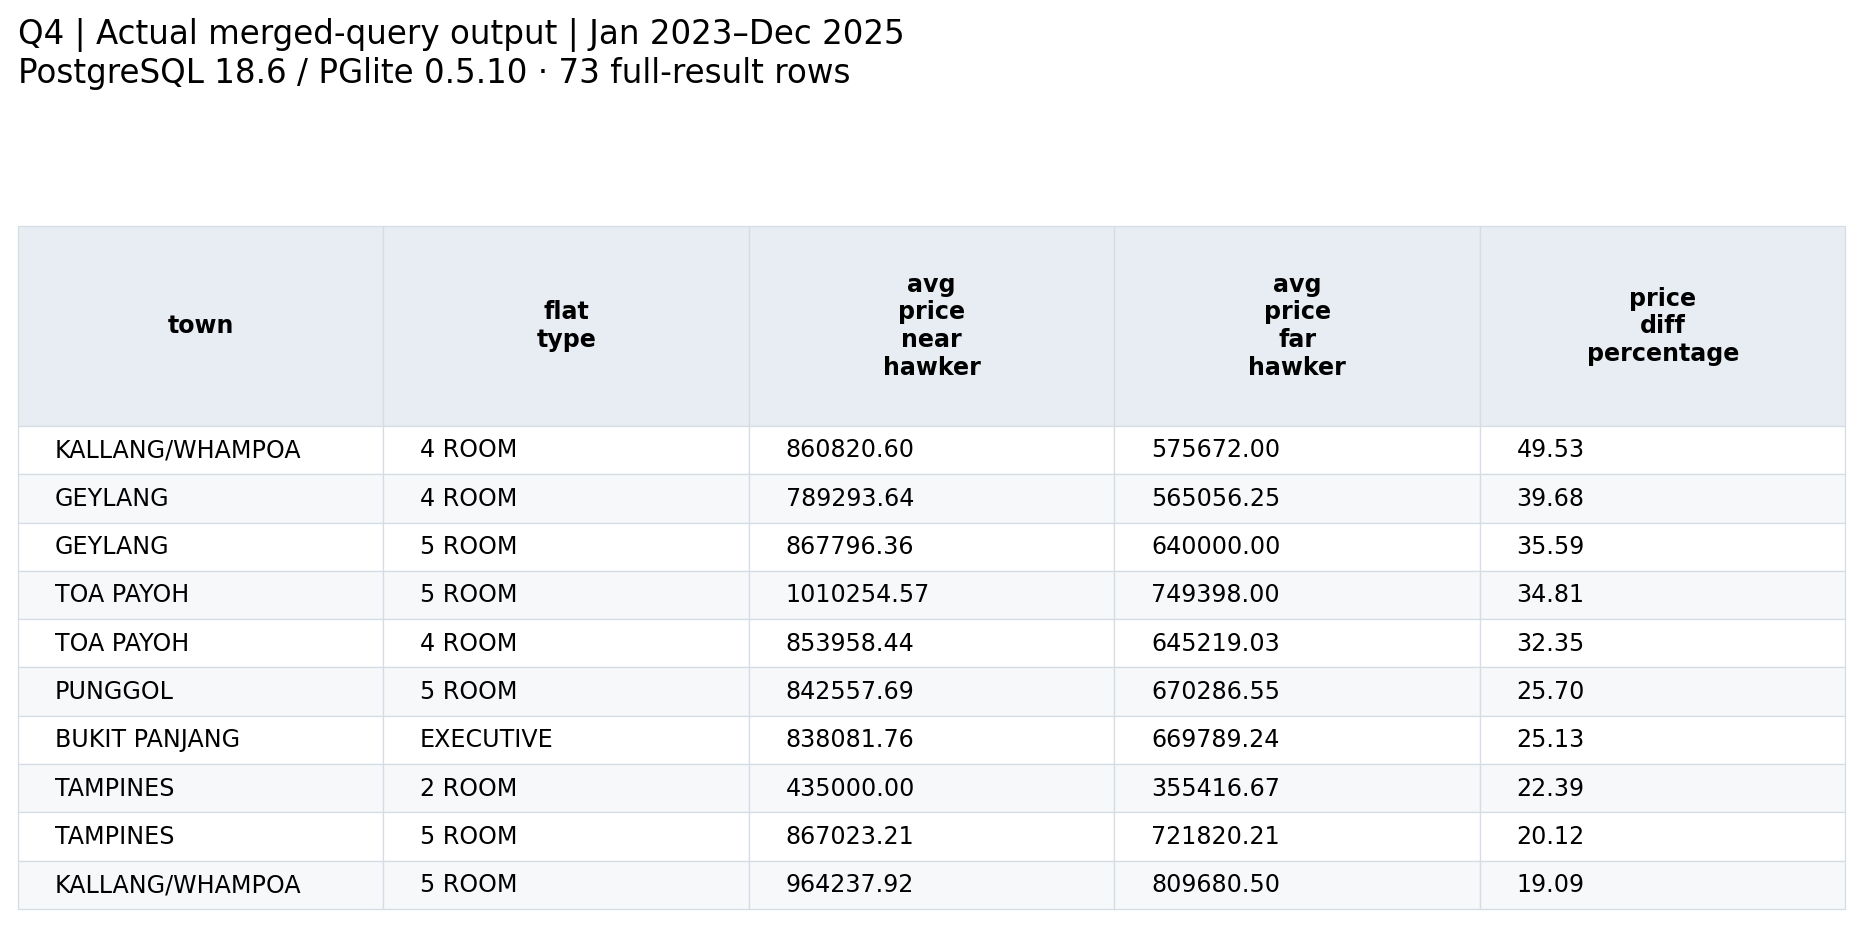
\includegraphics[width=0.94\linewidth,height=8.6cm,keepaspectratio]{../evidence/figures/Q4_result.png}
\caption{Q4 result excerpt: first ten of 73 groups by percentage difference.}\end{figure}
\begin{samepage}\textbf{Insight.} Kallang/Whampoa 4 ROOM has the largest positive difference: near SGD 860,820.60, far SGD 575,672.00, or 49.53\%. Across the 73 groups, 41 differences are positive and 32 negative. The mixed signs do not support a universal near-hawker premium. Housing mix, lease and other neighbourhood amenities remain potential confounders.\par\end{samepage}

\Needspace{10\baselineskip}\subsection{Q5: Prices near hawkers with fresh-market stalls}
\begin{samepage}An address qualifies for a class when it has at least one hawker with a positive fresh-market stall count in that class. Unknown status is excluded. The CTE makes each address/class pair unique before joining sales, so several qualifying centres do not multiply a sale within a group. The budget is fixed at \textbf{SGD 700,000} before timing and is unchanged across all five sizes. This three-year sample gives 11 passing town/class groups from 5 of 22 eligible towns. SGD 350,000 would select all 22 eligible towns in this sample.\par\end{samepage}

\Needspace{7\baselineskip}\lstinputlisting{../sql/queries/Q5.sql}
\begin{table}[H]\centering\small
\begin{tabular}{llrr}
\toprule
Town & Class & Mean SGD & Sales \\
\midrule
Bukit Timah & near & 897,986.20 & 162 \\
Bishan & medium & 848,219.63 & 886 \\
Bishan & far & 823,020.47 & 1,138 \\
Central Area & near & 805,810.01 & 450 \\
Central Area & medium & 787,059.31 & 495 \\
Central Area & far & 760,729.39 & 546 \\
Bukit Merah & near & 731,309.10 & 2,656 \\
Bukit Merah & far & 728,198.21 & 2,957 \\
Bukit Merah & medium & 717,838.37 & 2,424 \\
Queenstown & far & 712,094.01 & 1,902 \\
Queenstown & medium & 704,915.90 & 1,805 \\
\bottomrule
\end{tabular}
\caption{Q5: all 11 groups above the fixed SGD 700,000 budget, 2023-2025.}
\end{table}
\begin{table}[H]\centering\small
\begin{tabular}{lrrr}
\toprule
Size & Eligible towns & Passing towns & Groups \\
\midrule
S1 & 22 & 4 & 9 \\
S2 & 22 & 5 & 10 \\
S3 & 22 & 5 & 11 \\
S4 & 22 & 5 & 10 \\
S5 & 22 & 5 & 11 \\
\bottomrule
\end{tabular}
\caption{Q5: every measured size is nonempty and selects fewer than all eligible towns.}
\end{table}
\begin{figure}[H]\centering
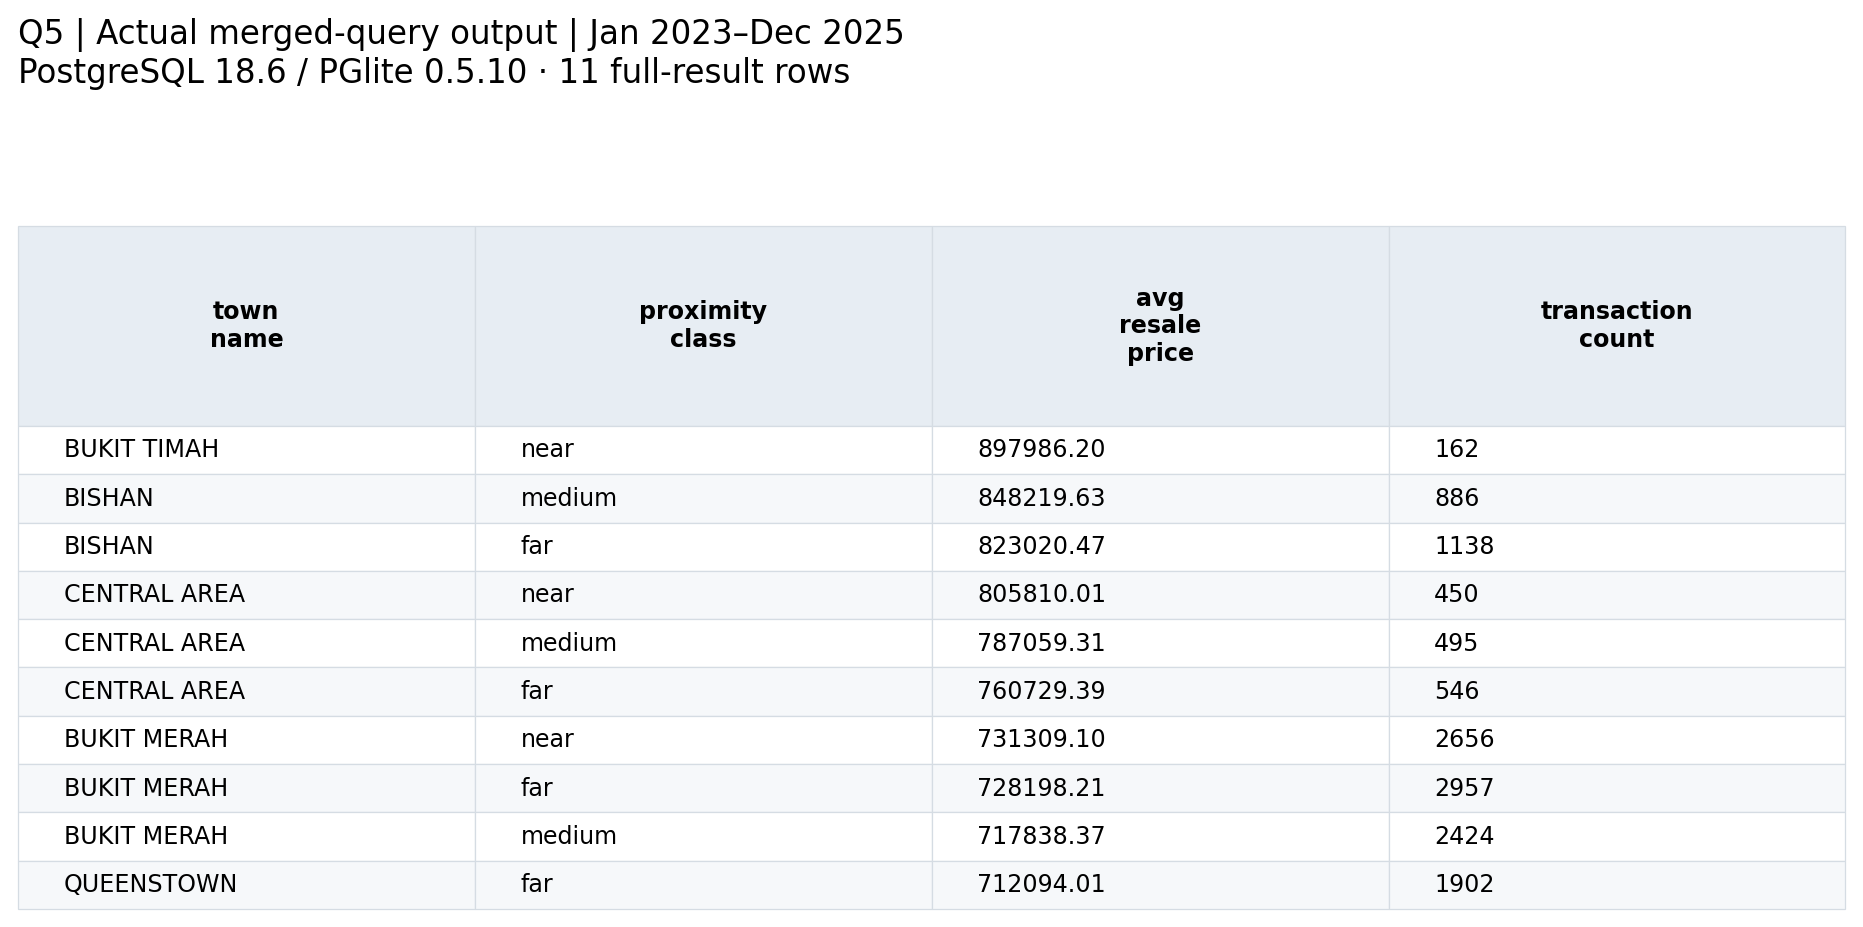
\includegraphics[width=0.94\linewidth,height=8.6cm,keepaspectratio]{../evidence/figures/Q5_result.png}
\caption{Q5 result excerpt: first ten of 11 passing groups, 2023-2025.}\end{figure}
\begin{samepage}\textbf{Insight.} Bukit Timah near has the highest passing mean, SGD 897,986.20, while Bishan medium and far also exceed SGD 800,000. High-price groups occur in different bands. A sale can belong to more than one class; group volumes therefore cannot be added to obtain a unique-sale total.\par\end{samepage}

\Needspace{10\baselineskip}\subsection{Q6: All-relation join}
\begin{samepage}The additional question asks how address coverage, transaction volume and mean price differ by town, distance band and fresh-market status. All six base relations participate explicitly, including the proximity lookup. Nearby, hawker and proximity memberships are deduplicated before joining town, address and transaction rows. Unique address/class/status memberships are formed before transactions are joined. The result contains 154 groups, including 57 groups with unknown market status. An address or sale may occur in several different groups, but only once within each group.\par\end{samepage}

\Needspace{7\baselineskip}\lstinputlisting{../sql/queries/Q6.sql}
\begin{table}[H]\centering\small
\begin{tabular}{lllrrr}
\toprule
Town & Class & Status & Addresses & Sales & Mean SGD \\
\midrule
Bukit Batok & near & unknown & 49 & 1,598 & 605,640.12 \\
Bukit Batok & medium & unknown & 112 & 801 & 563,789.31 \\
Bukit Batok & far & unknown & 225 & 1,988 & 572,255.17 \\
\bottomrule
\end{tabular}
\caption{Q6: Bukit Batok / unknown, all three distance groups within 2023-2025.}
\end{table}
\begin{figure}[H]\centering
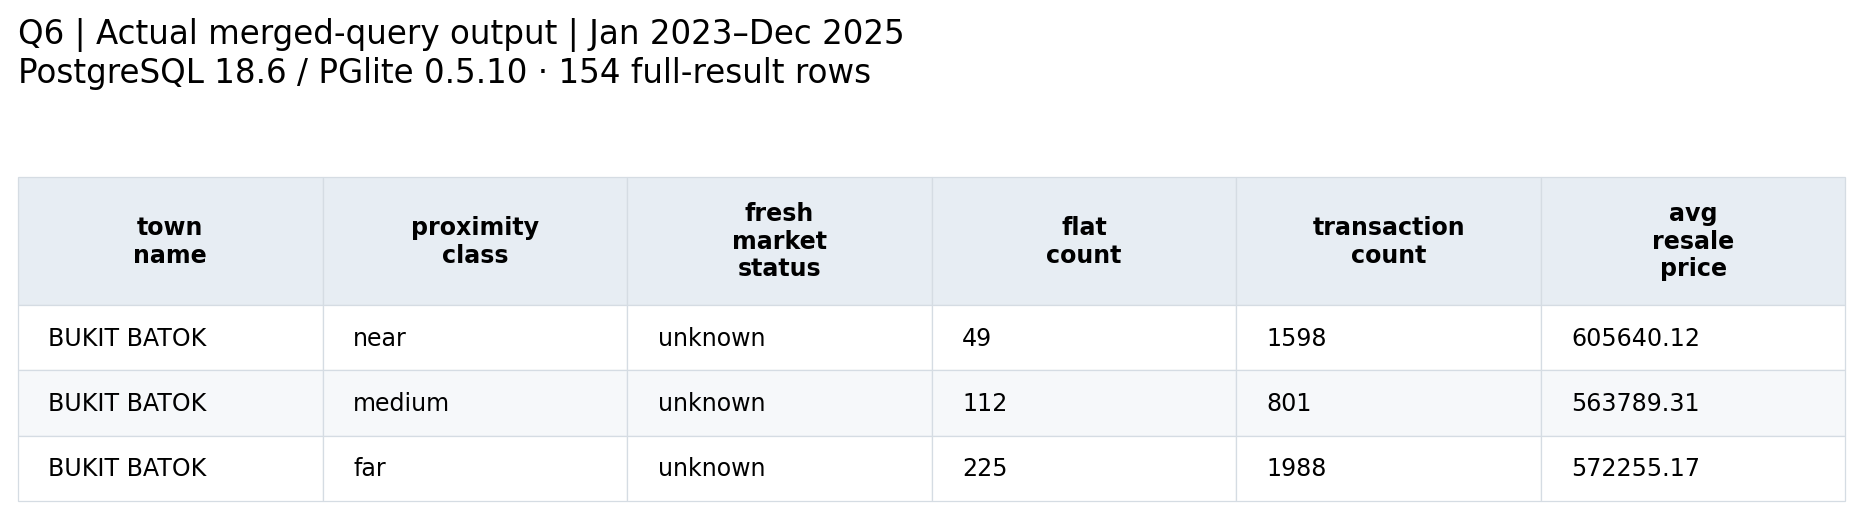
\includegraphics[width=0.94\linewidth,height=8.6cm,keepaspectratio]{../evidence/figures/Q6_result.png}
\caption{Q6 filtered excerpt: the same Bukit Batok / unknown groups shown in the table.}\end{figure}
\begin{samepage}\textbf{Insight.} Bukit Batok near/unknown contains 49 participating addresses and 1,598 sales, with mean SGD 605,640.12. Treating unknown as confirmed no would mislabel this population. Q6 pools all room types and accepts any matching centre in the band; Q4 uses a single nearest centre and separates room types. Their means therefore describe different populations, even with the same three-year date filter.\par\end{samepage}


\Needspace{10\baselineskip}\subsection{Merged-code performance measurements}
All five increasing sizes use the same 2023--2025 period. A stable source-row hash assigns each sale to one of five disjoint partitions: the first sixteen hexadecimal digits, interpreted as an integer, modulo five, plus one. The next partition is added at each size. All 36 months occur at every size; S5 contains every scoped transaction exactly once. Five reference relations remain fixed, including the three-row proximity lookup.

\textbf{Protocol scope.} The project guide's original five historical source-file increments differ from these within-period partitions. All selected 2023--2025 sales originate in the latest historical file. Approval of this revised protocol, or an additional experiment with the original five-file procedure, is required before claiming full compliance with that requirement.

\begin{table}[H]\centering\small
\begin{tabular}{lrrr}
\toprule
Size & Transactions & Months & Six-table MiB \\
\midrule
S1 & 15,640 & 36 & 9.68 \\
S2 & 31,581 & 36 & 14.88 \\
S3 & 47,295 & 36 & 19.48 \\
S4 & 63,007 & 36 & 24.39 \\
S5 & 78,670 & 36 & 29.03 \\
\bottomrule
\end{tabular}
\caption{Measured database footprints, including constraint indexes and TOAST, before analytical indexes.}
\end{table}

Each reference relation is bulk-loaded once. VACUUM (ANALYZE) precedes every transaction-size baseline; data and maintenance state remain fixed throughout Task 4. Primary-key, unique and exclusion indexes are retained. No optional analytical index exists in Task 3. Each complete SELECT is exported, warmed up once, and executed five measured times. Query order rotates cyclically. The metric is PostgreSQL Execution Time from EXPLAIN (ANALYZE, BUFFERS, TIMING OFF, FORMAT JSON); planning is recorded separately. Loading, output transfer and rendering are outside timing. No COUNT wrapper replaces the required SELECT.

\begin{table}[H]\centering\small
\begin{tabular}{lrrrrrr}
\toprule
Size & Q1 & Q2 & Q3 & Q4 & Q5 & Q6 \\
\midrule
S1 & 14.81 & 29.21 & 12.69 & 51.14 & 61.52 & 196.72 \\
S2 & 25.16 & 56.42 & 20.66 & 59.77 & 86.34 & 348.50 \\
S3 & 38.88 & 85.84 & 25.85 & 72.39 & 87.25 & 495.69 \\
S4 & 53.01 & 128.96 & 34.03 & 87.39 & 100.27 & 705.80 \\
S5 & 61.13 & 160.22 & 43.31 & 92.10 & 116.93 & 805.42 \\
\bottomrule
\end{tabular}
\caption{Mean executor milliseconds for the 150 fresh merged-code Task 3 observations.}
\end{table}

\begin{figure}[H]\centering
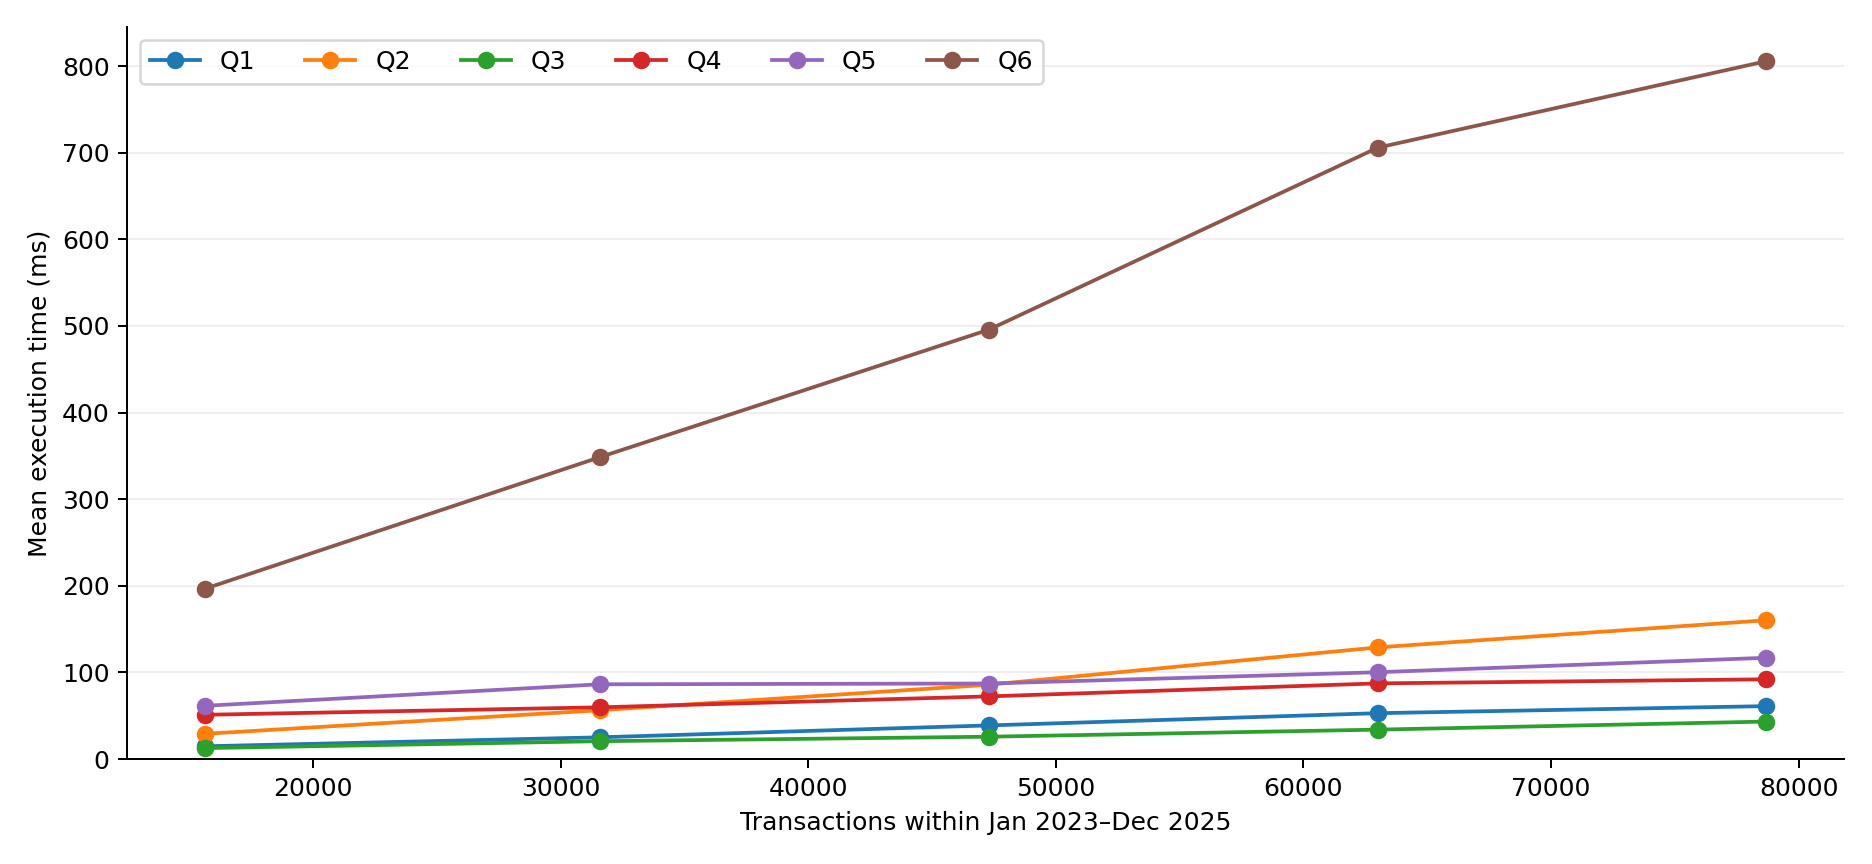
\includegraphics[width=0.95\linewidth]{../evidence/figures/Task3_scaling.png}
\caption{Fresh baseline means across five fixed-period cumulative populations.}\end{figure}

\textbf{Insight.} Q6 is the largest cost in this execution environment because its valid address/band/status memberships still expand into many sale memberships before grouping. Deduplicating membership before the transaction join protects correctness and reduces intermediate multiplication, but does not make the remaining aggregate selective. Sequential scans are reasonable for queries consuming most of the scoped population. These are measured scaling observations, not native disk-I/O or cross-machine claims.

\subsection{Integration and correctness checks}
The integration uses the teammate's six-relation lookup design and bulk-load approach, together with the scoped package's row keys, date constraints, nullable fresh-market status, fixed Q5 budget and independent validation. The uploaded SQL contributes the transaction-deduplication principle; the final Q5/Q6 form applies equivalent deduplication at the smaller address-membership grain. Q4 keeps deterministic nearest-centre selection. A single query-file set supplies displayed SQL, exported results and every benchmark configuration.

Independent pandas recomputation passes all six largest-data outputs: 52, 62, 30, 73, 11 and 154 groups. Every optional-index configuration produces the exact same complete output fingerprint as the S5 baseline. The common scope is 78,670 transactions and 36 months, with 40,354 stored and classified nearby links. The prior historical native timings and the uploaded 1997--1999 Q1 window are not reused as results for this instance.

\section{Task 4: Index Design and Experimental Evaluation}
\subsection{Objective and controlled protocol}
Task 4 selects indexes from actual EXPLAIN plans, runs each query five times on the largest Task 3 dataset, and compares indexed execution with that exact baseline. The deliverables include commented index DDL, raw observations, an Excel column chart, interpreted execution plans and reproducible scripts. This experiment uses 78,670 sales from January 2023 through December 2025; it does not mix the teammate's all-history population into the comparison.

The completed run contains 390 measured executions: 150 Task 3 baseline observations, 210 isolated candidate observations (seven configurations, six queries, five repeats), and 30 fresh confirmation observations. Each configuration has an excluded full-query warm-up and an untimed complete-result equality check. Data, SQL fingerprints, planner defaults and visibility maintenance remain unchanged. No index is forced by disabling sequential scans.

\textbf{Environment.} PostgreSQL 18.6 through PGlite 0.5.10, Node 24.22.1, Linux, Intel Xeon Platinum 8573C; nine logical CPUs are visible, while PostgreSQL parallel workers per gather are zero. Shared buffers are 128 MiB and work\_mem is 4 MiB. Storage is an in-memory WASM virtual filesystem. These actual timings are not a native PostgreSQL or physical-disk benchmark. The supplied native runner records the real server version and settings and repeats the full experiment in a new isolated schema.

\subsection{Plan-driven candidate design}
The baseline scans most transactions for Q1/Q2/Q4--Q6. Q3 filters the 3 ROOM subset twice. Q4 needs nearby rows ordered by address, distance and hawker ID. Q5/Q6 use address-centre memberships, and Q6 has a substantial grouping/sort workload. These observed operators motivate the following independent candidates.

\begin{table}[H]\centering\small
\begin{tabular}{lrrl}
\toprule
Isolated candidate & Geo. ratio & Index MiB & Used \\
\midrule
Date/type + address + lease & 0.957 & 1.875 & yes \\
Nearest-centre ordering & 1.196 & 1.570 & yes \\
3 ROOM partial covering & 1.142 & 0.766 & yes \\
4/5 ROOM partial covering & 1.001 & 2.492 & yes \\
Transaction address covering & 1.023 & 4.430 & yes \\
Reverse hawker membership & 1.032 & 1.570 & no \\
Town/address ordering & 1.002 & 0.297 & yes \\
\bottomrule
\end{tabular}
\caption{Exploratory ratio is the geometric mean of indexed/baseline mean times across Q1--Q6; below 1 is faster.}
\end{table}

The seven candidate DDL definitions are provided in \texttt{sql/05\_index\_candidates.json}; each statement has an explanatory trailing comment. Covering candidates include only projected/filter columns needed by their target queries. The 3 ROOM and 4/5 ROOM partial predicates match the corresponding query predicates. The nearest-order candidate matches Q4's deterministic ordering. The hawker-led and town-led alternatives test whether their join orders are useful rather than assuming that every foreign key needs an index for this analytical workload.

Index-only scans require both suitable index columns and visibility information. Equal VACUUM maintenance is therefore applied before baseline/index comparisons. The partial 3 ROOM trial actually uses two index-only scans with zero heap fetches, while the nearest-order trial eliminates Q4's incremental sort through an index-only scan. These plan improvements did not guarantee lower total six-query runtime in this environment. The reverse hawker index was not used. The town/address index was used but did not pass the aggregate selection criterion.

\subsection{Selection rule and confirmed index bundle}
The rule recorded before candidate evaluation retains a candidate group only when an actual plan uses one of its indexes and the equal-query-weight geometric mean ratio is below 0.98. Retained groups are recreated together and tested with five new repeats; individual gains are never added together. Only the teammate's three-index group passed the exploratory rule in this run. The fresh confirmation therefore measures precisely the following DDL.
\lstinputlisting{../evidence/run/selected_indexes.sql}

This is the confirmed experimental bundle, not a claim that three indexes are universally optimal. Within it, only \texttt{t4\_team\_month\_type} appears in the six-query plans. The address and lease indexes add storage/build/write cost without observed read benefit here. A practical deployment should test a pruned date/type-only bundle on native PostgreSQL before retaining those two unused indexes; its performance is not fabricated in this report. The selection rule evaluates candidate groups, so the measured three-index confirmation is preserved rather than silently relabelled as a one-index result.

\begin{table}[H]\centering\small
\begin{tabular}{lrrrrr}
\toprule
Query & Base mean & Base SD & Index mean & Index SD & Reduction \% \\
\midrule
Q1 & 61.13 & 3.74 & 66.59 & 4.96 & -8.93 \\
Q2 & 160.22 & 7.70 & 160.82 & 12.78 & -0.37 \\
Q3 & 43.31 & 5.89 & 31.54 & 2.25 & +27.16 \\
Q4 & 92.10 & 5.52 & 99.17 & 8.50 & -7.68 \\
Q5 & 116.93 & 15.44 & 112.19 & 7.79 & +4.05 \\
Q6 & 805.42 & 17.06 & 842.11 & 50.70 & -4.55 \\
\bottomrule
\end{tabular}
\caption{Largest-data executor times in milliseconds; five repeats and sample SD per query/configuration. Positive reduction means faster.}
\end{table}

\begin{figure}[H]\centering
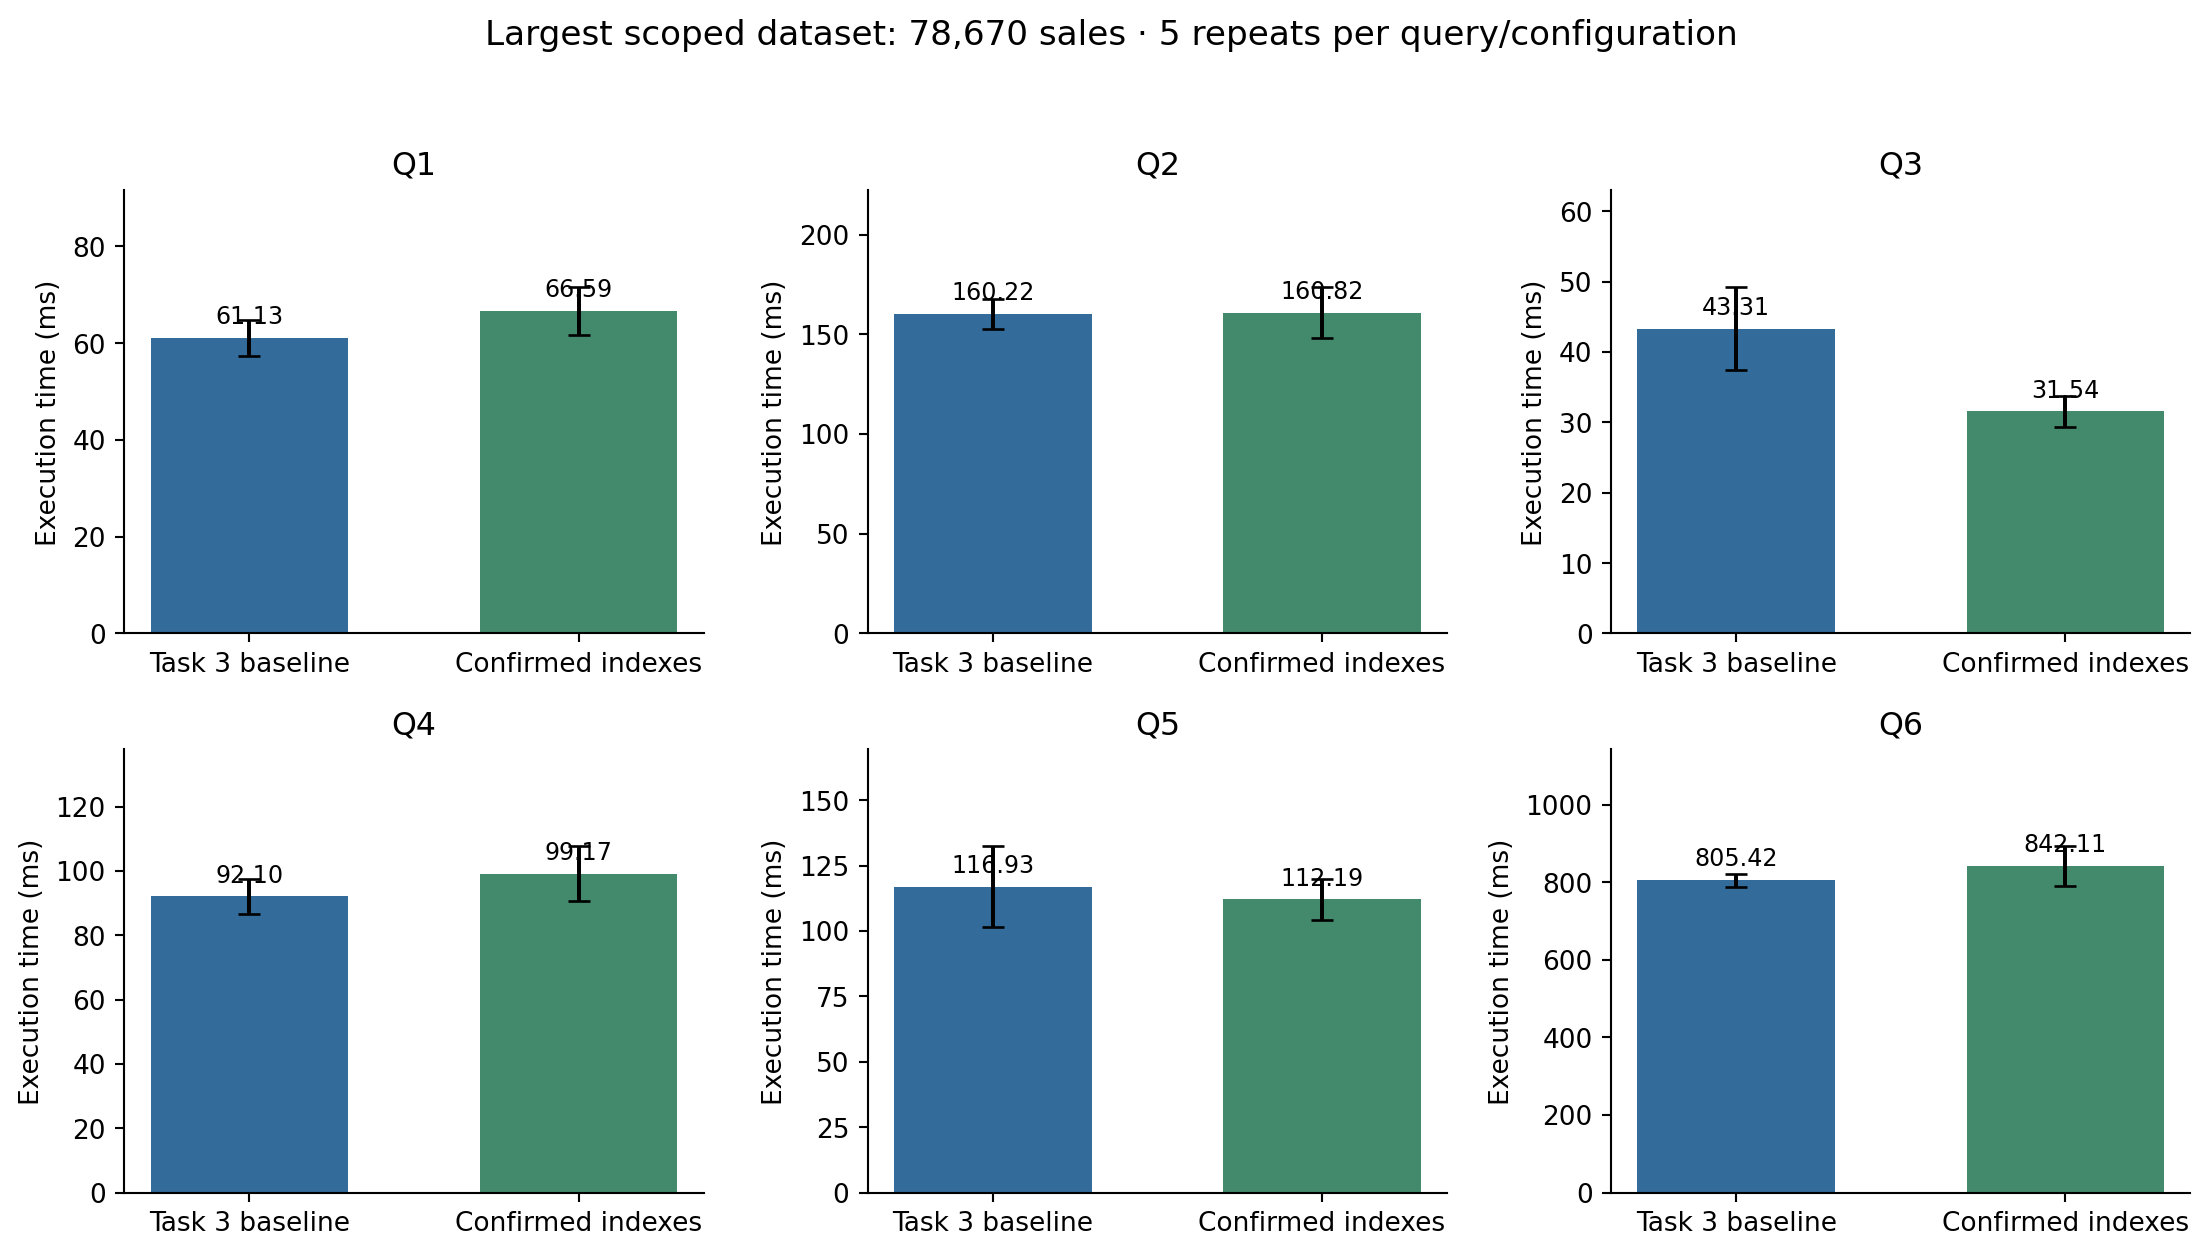
\includegraphics[width=0.95\linewidth]{../evidence/figures/Task4_comparison.png}
\caption{Task 3 S5 baseline versus the fresh confirmed bundle. Bars show means; error bars show sample SD. Every panel begins at zero.}\end{figure}
\textbf{Insight.} Q3 falls from 43.31 ms to 31.54 ms, a 27.16\% reduction. Q1, Q2, Q4 and Q6 are slower in the confirmation, while Q5 is slightly faster. The confirmation geometric mean ratio is 0.975; the sum of six mean times changes from 1279.12 to 1312.42 ms (-2.60\% reduction). The equal-query ratio suggests a modest improvement, while the sum of query means regresses; these two weightings must not be confused. This does not establish a uniformly faster workload. Five warm repeats on one host do not establish statistical significance.

\begin{table}[H]\centering\small
\begin{tabular}{lrrrrr}
\toprule
Query & Base R1 & Base R2 & Base R3 & Base R4 & Base R5 \\
\midrule
Q1 & 60.798 & 59.001 & 67.164 & 61.422 & 57.287 \\
Q2 & 165.260 & 154.585 & 171.356 & 155.590 & 154.329 \\
Q3 & 39.511 & 51.645 & 41.720 & 46.724 & 36.940 \\
Q4 & 83.462 & 93.683 & 91.356 & 98.605 & 93.414 \\
Q5 & 109.096 & 105.273 & 135.843 & 131.335 & 103.098 \\
Q6 & 805.910 & 785.182 & 829.821 & 811.689 & 794.503 \\
\bottomrule
\end{tabular}
\caption{All five raw largest-data baseline times (ms); repetition identity follows the raw CSV.}
\end{table}

\begin{table}[H]\centering\small
\begin{tabular}{lrrrrr}
\toprule
Query & Index R1 & Index R2 & Index R3 & Index R4 & Index R5 \\
\midrule
Q1 & 69.950 & 59.888 & 72.695 & 64.473 & 65.948 \\
Q2 & 163.303 & 156.445 & 180.760 & 157.555 & 146.013 \\
Q3 & 29.619 & 30.270 & 30.144 & 34.913 & 32.778 \\
Q4 & 92.233 & 98.530 & 96.049 & 113.830 & 95.229 \\
Q5 & 109.967 & 112.220 & 125.042 & 109.663 & 104.049 \\
Q6 & 805.820 & 926.672 & 834.612 & 843.220 & 800.206 \\
\bottomrule
\end{tabular}
\caption{All five raw fresh confirmation times (ms).}
\end{table}

\subsection{What the execution plans establish}
Q3's baseline scans transactions twice. The confirmed plan instead uses \texttt{t4\_team\_month\_type} bitmap index scans in both branches, each identifying 19,297 3 ROOM sales. This operator change supports the measured improvement. The date range covers all stored sales, so it is not selective; room type provides the filtering opportunity. A type-led or partial alternative remains worth testing on the intended native workload.

Q2's remaining-lease CASE expression classifies all transactions rather than searching a narrow lease interval. The lease index is unused. Q1 consumes 52,280 4/5 ROOM sales, and Q4--Q6 retain broad cohorts; none uses the confirmed optional indexes. Their output ordering and aggregates still cost work. Q4 continues to read the nearby primary-key index with an incremental sort; the separate nearest-order candidate changes that plan, but its measured total runtime does not justify claiming an overall improvement. Q6 sorts 195,690 sale-membership rows in the representative largest-data baseline. It remains dominated by membership expansion and aggregation, not a selective transaction lookup.

The relevant complete plans are stored under \texttt{evidence/run/plans}; compact node summaries and index inventories are under \texttt{evidence/run/configurations}. They record actual row counts, loops, heap fetches, buffers and sort details. A created index is considered used only when its name appears in an actual plan.

The confirmed three-index bundle occupies 1.875 MiB and takes 162.57 ms of separate build wall time in this run. Build time is not included in SELECT timings. Extra indexes also require maintenance during future inserts and updates; the read-only experiment does not quantify that write penalty.

\subsection{Deliverables and reproduction}
\texttt{SD6103\_Task4\_Results.xlsx} contains a formula-driven Summary sheet with an editable Excel bar chart, a Candidates sheet retaining all seven trials, and a Raw sheet containing all 390 observations. Means, sample deviations and reductions are calculated from raw measurements. The full raw CSV, SQL fingerprints, complete outputs, all timed plans, candidate outcomes and final index DDL accompany the workbook.

Annotated reproduction commands and dependency setup are in the package README. Both runners require an empty output folder. The native runner retains a fresh schema, repeats all trials, and selects indexes from native measurements. The macOS launcher supplies portable demo-database defaults.

\textbf{Submission boundary.} The merged queries, independent result checks and scoped WASM experiment are complete. Confirm acceptance of the 2023--2025 partition protocol and alternative tool, or run the prescribed historical-file/native procedure. Genuine pgAdmin captures must come from the native run when required; supplied figures are labelled result exports.

\subsection{References and provenance}
PostgreSQL 18 documentation: \url{https://www.postgresql.org/docs/18/sql-explain.html}; index-only scans, \url{https://www.postgresql.org/docs/18/indexes-index-only-scans.html}; partial indexes, \url{https://www.postgresql.org/docs/18/indexes-partial.html}.

Teammate source: \url{https://github.com/yzxfwdplf/SD6103-Data-Systems-Task3}. The archived snapshot records file-level blob SHAs and URLs, with the root tree labelled separately. Uploaded SQL, scoped-data manifests and validation evidence are preserved in the package.

\end{document}
